% !TeX spellcheck = hu_HU
% !TeX encoding = UTF-8
% !TeX program = xelatex
\documentclass[11pt,a4paper,oneside]{report}             % Single-side
%\documentclass[11pt,a4paper,twoside,openright]{report}  % Duplex

% thanks to http://tex.stackexchange.com/a/47579/71109
\usepackage{ifxetex}
\usepackage{ifluatex}
\newif\ifxetexorluatex % a new conditional starts as false
\ifnum 0\ifxetex 1\fi\ifluatex 1\fi>0
   \xetexorluatextrue
\fi

\ifxetexorluatex
  \usepackage{fontspec}
\else
  \usepackage[T1]{fontenc}
  \usepackage[utf8]{inputenc}
  \usepackage[lighttt]{lmodern}
\fi

\usepackage[english,magyar]{babel} % Alapértelmezés szerint utoljára definiált nyelv lesz aktív, de később külön beállítjuk az aktív nyelvet.

%\usepackage{cmap}
\usepackage{amsfonts,amsmath,amssymb} % Mathematical symbols.
%\usepackage[ruled,boxed,resetcount,linesnumbered]{algorithm2e} % For pseudocodes. % beware: this is not compatible with LuaLaTeX, see http://tex.stackexchange.com/questions/34814/lualatex-and-algorithm2e
\usepackage{booktabs} % For publication quality tables for LaTeX
\usepackage{graphicx}

%\usepackage{fancyhdr}
%\usepackage{lastpage}

\usepackage{anysize}
%\usepackage{sectsty}
\usepackage{setspace} % For setting line spacing

\usepackage[unicode]{hyperref} % For hyperlinks in the generated document.
\usepackage{xcolor}
\usepackage{listings} % For source code snippets.

\usepackage[amsmath,thmmarks]{ntheorem} % Theorem-like environments.

\usepackage[hang]{caption}

\singlespacing

\newcommand{\selecthungarian}{
	\selectlanguage{magyar}
	\setlength{\parindent}{2em}
	\setlength{\parskip}{0em}
	\frenchspacing
}

\newcommand{\selectenglish}{
	\selectlanguage{english}
	\setlength{\parindent}{0em}
	\setlength{\parskip}{0.5em}
	\nonfrenchspacing
	\renewcommand{\figureautorefname}{Figure}
	\renewcommand{\tableautorefname}{Table}
	\renewcommand{\partautorefname}{Part}
	\renewcommand{\chapterautorefname}{Chapter}
	\renewcommand{\sectionautorefname}{Section}
	\renewcommand{\subsectionautorefname}{Section}
	\renewcommand{\subsubsectionautorefname}{Section}
}

\usepackage[numbers]{natbib}
\usepackage{xspace}


\newcommand{\vikszerzoVezeteknev}{Putovici}
\newcommand{\vikszerzoKeresztnev}{Ábel}

\newcommand{\vikkonzulensAMegszolitas}{}
\newcommand{\vikkonzulensAVezeteknev}{Paróczi}
\newcommand{\vikkonzulensAKeresztnev}{Zsombor}

\newcommand{\vikkonzulensBMegszolitas}{}
\newcommand{\vikkonzulensBVezeteknev}{}
\newcommand{\vikkonzulensBKeresztnev}{}

\newcommand{\vikkonzulensCMegszolitas}{}
\newcommand{\vikkonzulensCVezeteknev}{}
\newcommand{\vikkonzulensCKeresztnev}{}

\newcommand{\vikcim}{DHT használata WebRTC signaling megvalósításához} % Cím
\newcommand{\viktanszek}{\bmetmit} % Tanszék
\newcommand{\vikdoktipus}{\msconlabii} % Dokumentum típusa (\bsc vagy \msc)
\newcommand{\vikmunkatipusat}{szakdolgozatot} % a "hallgató nyilatkozat" részhez: szakdolgozatot vagy diplomatervet

%--------------------------------------------------------------------------------------
% TDK-specifikus változók
%--------------------------------------------------------------------------------------
\newcommand{\tdkszerzoB}{Második Szerző} % Második szerző neve; hagyd üresen, ha egyedül írtad a TDK-t.
\newcommand{\tdkev}{2014} % A dolgozat írásának éve (pl. "2014") (Ez OTDK-nál eltérhet az aktuális évtől.)

% További adatok az OTDK címlaphoz (BME-s TDK-hoz nem kell kitölteni)
\newcommand{\tdkevfolyamA}{IV} % Első szerző évfolyama, római számmal (pl. IV).
\newcommand{\tdkevfolyamB}{III} % Második szerző évfolyama, római számmal (pl. III).
\newcommand{\tdkkonzulensbeosztasA}{egyetemi tanár} % Első konzulens beosztása (pl. egyetemi docens)
\newcommand{\tdkkonzulensbeosztasB}{doktorandusz} % Második konzulens beosztása (pl. egyetemi docens)

\newcommand{\szerzoMeta}{\vikszerzoVezeteknev{} \vikszerzoKeresztnev} % egy szerző esetén
%\newcommand{\szerzoMeta}{\vikszerzoVezeteknev{} \vikszerzoKeresztnev, \tdkszerzoB} % két szerző esetén

% Beállítások magyar nyelvű dolgozathoz
%--------------------------------------------------------------------------------------
% Elnevezések
%--------------------------------------------------------------------------------------
\newcommand{\bme}{Budapesti Műszaki és Gazdaságtudományi Egyetem}
\newcommand{\vik}{Villamosmérnöki és Informatikai Kar}

\newcommand{\bmemit}{Méréstechnika és Információs Rendszerek Tanszék}
\newcommand{\bmetmit}{Távközlési és Médiainformatikai Tanszék}

\newcommand{\keszitette}{Készítette}
\newcommand{\konzulens}{Konzulens}

\newcommand{\bsc}{Szakdolgozat}
\newcommand{\msc}{Diplomaterv}
\newcommand{\tdk}{TDK dolgozat}
\newcommand{\bsconlab}{BSc Önálló laboratórium}
\newcommand{\msconlabi}{MSc Önálló laboratórium 1.}
\newcommand{\msconlabii}{MSc Önálló laboratórium 2.}

\newcommand{\pelda}{Példa}
\newcommand{\definicio}{Definíció}
\newcommand{\tetel}{Tétel}

\newcommand{\bevezetes}{Bevezetés}
\newcommand{\koszonetnyilvanitas}{Köszönetnyilvánítás}
\newcommand{\fuggelek}{Függelék}

% Opcionálisan átnevezhető címek
%\addto\captionsmagyar{%
%\renewcommand{\listfigurename}{Saját ábrajegyzék cím}
%\renewcommand{\listtablename}{Saját táblázatjegyzék cím}
%\renewcommand{\bibname}{Saját irodalomjegyzék név}
%}

\newcommand{\szerzo}{\vikszerzoVezeteknev{} \vikszerzoKeresztnev}
\newcommand{\vikkonzulensA}{\vikkonzulensAMegszolitas\vikkonzulensAVezeteknev{} \vikkonzulensAKeresztnev}
\newcommand{\vikkonzulensB}{\vikkonzulensBMegszolitas\vikkonzulensBVezeteknev{} \vikkonzulensBKeresztnev}
\newcommand{\vikkonzulensC}{\vikkonzulensCMegszolitas\vikkonzulensCVezeteknev{} \vikkonzulensCKeresztnev}

\newcommand{\selectthesislanguage}{\selecthungarian}

\bibliographystyle{huplain}

\def\lstlistingname{lista}

\newcommand{\appendixnumber}{6}  % a fofejezet-szamlalo az angol ABC 6. betuje (F) lesz

% Settings for English documents
%%--------------------------------------------------------------------------------------
% Elnevezések
%--------------------------------------------------------------------------------------
\newcommand{\bme}{Budapest University of Technology and Economics}
\newcommand{\vik}{Faculty of Electrical Engineering and Informatics}

\newcommand{\bmemit}{Department of Measurement and Information Systems}

\newcommand{\keszitette}{Author}
\newcommand{\konzulens}{Advisor}

\newcommand{\bsc}{Bachelor's Thesis}
\newcommand{\msc}{Master's Thesis}
\newcommand{\tdk}{Scientific Students' Association Report}
\newcommand{\bsconlab}{BSc Project Laboratory}
\newcommand{\msconlabi}{MSc Project Laboratory 1}
\newcommand{\msconlabii}{MSc Project Laboratory 2}

\newcommand{\pelda}{Example}
\newcommand{\definicio}{Definition}
\newcommand{\tetel}{Theorem}

\newcommand{\bevezetes}{Introduction}
\newcommand{\koszonetnyilvanitas}{Acknowledgements}
\newcommand{\fuggelek}{Appendix}

% Optional custom titles
%\addto\captionsenglish{%
%\renewcommand*{\listfigurename}{Your list of figures title}
%\renewcommand*{\listtablename}{Your list of tables title}
%\renewcommand*{\bibname}{Your bibliography title}
%}

\newcommand{\szerzo}{\vikszerzoKeresztnev{} \vikszerzoVezeteknev}
\newcommand{\vikkonzulensA}{\vikkonzulensAMegszolitas\vikkonzulensAKeresztnev{} \vikkonzulensAVezeteknev}
\newcommand{\vikkonzulensB}{\vikkonzulensBMegszolitas\vikkonzulensBKeresztnev{} \vikkonzulensBVezeteknev}
\newcommand{\vikkonzulensC}{\vikkonzulensCMegszolitas\vikkonzulensCKeresztnev{} \vikkonzulensCVezeteknev}

\newcommand{\selectthesislanguage}{\selectenglish}

\bibliographystyle{plainnat}

\newcommand{\ie}{i.e.\@\xspace}
\newcommand{\Ie}{I.e.\@\xspace}
\newcommand{\eg}{e.g.\@\xspace}
\newcommand{\Eg}{E.g.\@\xspace}
\newcommand{\etal}{et al.\@\xspace}
\newcommand{\etc}{etc.\@\xspace}
\newcommand{\vs}{vs.\@\xspace}
\newcommand{\viz}{viz.\@\xspace} % videlicet
\newcommand{\cf}{cf.\@\xspace} % confer
\newcommand{\Cf}{Cf.\@\xspace}
\newcommand{\wrt}{w.r.t.\@\xspace} % with respect to
\newcommand{\approximately}{approx.\@\xspace}

\newcommand{\appendixnumber}{1}  % a fofejezet-szamlalo az angol ABC 1. betuje (A) lesz


%--------------------------------------------------------------------------------------
% Page layout setup
%--------------------------------------------------------------------------------------
% we need to redefine the pagestyle plain
% another possibility is to use the body of this command without \fancypagestyle
% and use \pagestyle{fancy} but in that case the special pages
% (like the ToC, the References, and the Chapter pages)remain in plane style

\pagestyle{plain}
\marginsize{35mm}{25mm}{15mm}{15mm}

\setcounter{tocdepth}{3}
%\sectionfont{\large\upshape\bfseries}
\setcounter{secnumdepth}{3}

\sloppy % Margón túllógó sorok tiltása.
\widowpenalty=10000 \clubpenalty=10000 %A fattyú- és árvasorok elkerülése
\def\hyph{-\penalty0\hskip0pt\relax} % Kötőjeles szavak elválasztásának engedélyezése


%--------------------------------------------------------------------------------------
% Setup hyperref package
%--------------------------------------------------------------------------------------
\hypersetup{
    % bookmarks=true,            % show bookmarks bar?
    unicode=true,              % non-Latin characters in Acrobat's bookmarks
    pdftitle={\vikcim},        % title
    pdfauthor={\szerzoMeta},    % author
    pdfsubject={\vikdoktipus}, % subject of the document
    pdfcreator={\szerzoMeta},   % creator of the document
    pdfproducer={},    % producer of the document
    pdfkeywords={},    % list of keywords (separate then by comma)
    pdfnewwindow=true,         % links in new window
    colorlinks=true,           % false: boxed links; true: colored links
    linkcolor=black,           % color of internal links
    citecolor=black,           % color of links to bibliography
    filecolor=black,           % color of file links
    urlcolor=black             % color of external links
}


%--------------------------------------------------------------------------------------
% Set up listings
%--------------------------------------------------------------------------------------
\definecolor{lightgray}{rgb}{0.95,0.95,0.95}
\lstset{
	basicstyle=\scriptsize\ttfamily, % print whole listing small
	keywordstyle=\color{black}\bfseries, % bold black keywords
	identifierstyle=, % nothing happens
	% default behavior: comments in italic, to change use
	% commentstyle=\color{green}, % for e.g. green comments
	stringstyle=\scriptsize,
	showstringspaces=false, % no special string spaces
	aboveskip=3pt,
	belowskip=3pt,
	backgroundcolor=\color{lightgray},
	columns=flexible,
	keepspaces=true,
	escapeinside={(*@}{@*)},
	captionpos=b,
	breaklines=true,
	frame=single,
	float=!ht,
	tabsize=2,
	literate=*
		{á}{{\'a}}1	{é}{{\'e}}1	{í}{{\'i}}1	{ó}{{\'o}}1	{ö}{{\"o}}1	{ő}{{\H{o}}}1	{ú}{{\'u}}1	{ü}{{\"u}}1	{ű}{{\H{u}}}1
		{Á}{{\'A}}1	{É}{{\'E}}1	{Í}{{\'I}}1	{Ó}{{\'O}}1	{Ö}{{\"O}}1	{Ő}{{\H{O}}}1	{Ú}{{\'U}}1	{Ü}{{\"U}}1	{Ű}{{\H{U}}}1
}


%--------------------------------------------------------------------------------------
% Set up theorem-like environments
%--------------------------------------------------------------------------------------
% Using ntheorem package -- see http://www.math.washington.edu/tex-archive/macros/latex/contrib/ntheorem/ntheorem.pdf

\theoremstyle{plain}
\theoremseparator{.}
\newtheorem{example}{\pelda}

\theoremseparator{.}
%\theoremprework{\bigskip\hrule\medskip}
%\theorempostwork{\hrule\bigskip}
\theorembodyfont{\upshape}
\theoremsymbol{{\large \ensuremath{\centerdot}}}
\newtheorem{definition}{\definicio}

\theoremseparator{.}
%\theoremprework{\bigskip\hrule\medskip}
%\theorempostwork{\hrule\bigskip}
\newtheorem{theorem}{\tetel}


%--------------------------------------------------------------------------------------
% Some new commands and declarations
%--------------------------------------------------------------------------------------
\newcommand{\code}[1]{{\upshape\ttfamily\scriptsize\indent #1}}
\newcommand{\doi}[1]{DOI: \href{http://dx.doi.org/\detokenize{#1}}{\raggedright{\texttt{\detokenize{#1}}}}} % A hivatkozások közt így könnyebb DOI-t megadni.

\DeclareMathOperator*{\argmax}{arg\,max}
%\DeclareMathOperator*[1]{\floor}{arg\,max}
\DeclareMathOperator{\sign}{sgn}
\DeclareMathOperator{\rot}{rot}


%--------------------------------------------------------------------------------------
% Setup captions
%--------------------------------------------------------------------------------------
\captionsetup[figure]{
	width=.75\textwidth,
	aboveskip=10pt}

\renewcommand{\captionlabelfont}{\bf}
%\renewcommand{\captionfont}{\footnotesize\it}

%--------------------------------------------------------------------------------------
% Hyphenation exceptions
%--------------------------------------------------------------------------------------
\hyphenation{Shakes-peare Mar-seilles ár-víz-tű-rő tü-kör-fú-ró-gép}


\author{\vikszerzo}
\title{\viktitle}

%--------------------------------------------------------------------------------------
% Table of contents and the main text
%--------------------------------------------------------------------------------------
\begin{document}

    \pagenumbering{gobble}

    \selectthesislanguage

%~~~~~~~~~~~~~~~~~~~~~~~~~~~~~~~~~~~~~~~~~~~~~~~~~~~~~~~~~~~~~~~~~~~~~~~~~~~~~~~~~~~~~~
    \hypersetup{pageanchor=false}
%--------------------------------------------------------------------------------------
%	The title page
%--------------------------------------------------------------------------------------
\begin{titlepage}
\begin{center}

\includegraphics[width=60mm,keepaspectratio]{figures/bme_logo.pdf}\\
\vspace{0.3cm}
\textbf{\bme}\\
\textmd{\vik}\\
\textmd{\viktanszek}\\[5cm]

\vspace{0.4cm}
{\huge \bfseries \vikcim}\\[0.8cm]
\vspace{0.5cm}
\textsc{\Large \vikdoktipus}\\[4cm]

{
	\renewcommand{\arraystretch}{0.85}
	\begin{tabular}{cc}
	 \makebox[7cm]{\emph{\keszitette}} & \makebox[7cm]{\emph{\konzulens}} \\ \noalign{\smallskip}
	 \makebox[7cm]{\szerzo} & \makebox[7cm]{\vikkonzulensA} \\
	  & \makebox[7cm]{\vikkonzulensB} \\
	  & \makebox[7cm]{\vikkonzulensC} \\
	\end{tabular}
}

\vfill
{\large \today}
\end{center}
\end{titlepage}
\hypersetup{pageanchor=false}

           % Szakdolgozat/Diplomaterv címlap
    %--------------------------------------------------------------------------------------
% Feladatkiiras (a tanszeken atveheto, kinyomtatott valtozat)
%--------------------------------------------------------------------------------------
\clearpage
\begin{center}
    \large
    \textbf{FELADATKIÍRÁS}\\
\end{center}

A hallgató feladata egy olyan algoritmus meghatározása, amely lehetővé teszi a WebRTC peer-ek közötti signaling folyamat
megvalósítását elosztott hash-táblák (DHT) segítségével.
Az algoritmus célja két WebRTC peer közötti csatlakozás létrehozása, a hallgató ennek működését egy proof-of-concept
implementációval mutatja be.
A hallgató feladata továbbá, hogy dolgozatában vizsgálja az algoritmus továbbfejlesztési lehetőségeit egy több peer-ből
álló WebRTC hálózat felépítésének érdekében.


% Table of Contents
%~~~~~~~~~~~~~~~~~~~~~~~~~~~~~~~~~~~~~~~~~~~~~~~~~~~~~~~~~~~~~~~~~~~~~~~~~~~~~~~~~~~~~~
    \tableofcontents\vfill

% The main part of the thesis
%~~~~~~~~~~~~~~~~~~~~~~~~~~~~~~~~~~~~~~~~~~~~~~~~~~~~~~~~~~~~~~~~~~~~~~~~~~~~~~~~~~~~~~
    \pagenumbering{arabic}

    %----------------------------------------------------------------------------
\chapter{\bevezetes}\label{ch:bevezetes}
%----------------------------------------------------------------------------


\section{A WebRTC protokoll}\label{sec:a-webrtc-protokoll}

Napjainkban a SaaS (Software-as-a-Service) típusú szolgáltatásokra nagy mértékben jellemző a centralizáltság, elosztott
rendszerek esetében is: a felhasználók az esetek többségében egy menedzselt környezetben futó, globálisan
elérhető szerveren (legyen ez egy load balancer vagy egy egyszerű ingress-jellegű reverse proxy) keresztül lépnek
interakcióba a rendszerrel.
A centralizált jelleg a minőségbiztosítás megkönnyítése mellett hordoz egy elhanyagolhatatlan negatívumot is: ha az előbb
említett globálisan elérhető szerver meghibásodik, akkor a végfelhasználók nem tudják elérni a rendszert, hiába működik
ez hibátlanul.

Az IPv6 bevezetése és folyamatos elterjedése ugyanakkor lehetőséget biztosít arra, hogy másképp tekintsünk az internetre:
egy olyan kommunikációs hálózat, ahol akár a végfelhasználók számítógépei is képesek közvetlenül egymással kommunikálni,
NAT szüksége nélkül.

A WebRTC (RFC 7478\cite{RFC_7478}) egy olyan kommunikációs protokoll, amely lehetővé teszi két vagy több résztvevő közötti hang- és
videóhívások, illetve általános célú adatcsere megvalósítását egy köztes fél jelenléte nélkül.
Mivel a videóhívások meglehetősen széles sávszélességet igényelhetnek, a protokoll csökkenti annak az esélyét,
hogy egy köztes fél szűk keresztmetszetté váljon ennek végessége miatt.

Az előző félév Önálló Laboratóriumának keretein belül is a WebRTC protokollal foglalkoztam, ahol az elosztott nyomkövetés
problémájára kerestem egy alternatív megoldást.
Ebben a dolgozatban a protokoll használata során implementálandó signaling folyamatra keresek egy decentralizált, köztes
fél nélkül működő megoldást.

A protokoll használata során az egyes felek lehetőség szerint közvetlenül egymással kommunikálnak, peer-to-peer módon.
A kommunikációs csatorna az ICE (RFC 8445\cite{ICE}) protokoll használatával van felépítve, amely során a felek egy STUN (RFC 5389)
szerver segítségével felderítik a saját publikus IP címüket és olyan port-ot, amelyen globálisan elérhetőek.
Amennyiben valamely fél olyan NAT környezetben van, amelyben nem valósítható meg a peer-to-peer kommunikáció, mint például
a szimmetrikus NAT típusok, a két fél egy köztes TURN (RFC 5766\cite{TURN}) szerveren keresztül kommunikál egymással, amely egy
relay-jellegű funkcionalitást valósít meg.
Az~\ref{fig:ice}-es ábra az ICE protokoll működését mutatja be.

\begin{figure}[!ht]
    \centering
    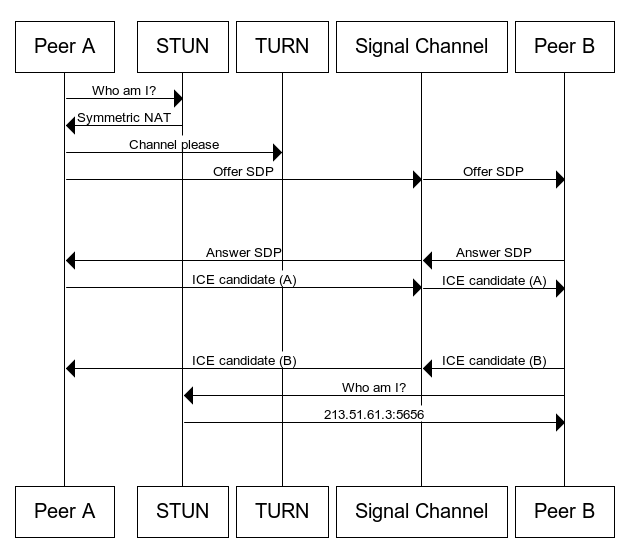
\includegraphics[width=150mm, keepaspectratio]{figures/ice}
    \caption{Az ICE folyamat ábrázolva (forrás: \href{https://developer.mozilla.org/en-US/docs/Web/API/WebRTC_API/Connectivity}{developer.mozilla.org})}
    \label{fig:ice}
\end{figure}

A kommunikáció felépítésének (más néven \emph{signaling}) során szükség van egy out-of-band, \textbf{kétirányú}
kommunikációs csatornára, amelyen keresztül a résztvevők elküldik egymásnak az ICE folyamat során szerzett ICE candidate-eket.
Ezt a csatornát a WebRTC protokoll \emph{nem biztosítja}.
A gyakorlatban ez a csatorna általában a WebSocket protokoll (RFC 6455\cite{WebSocket}) használatával, vagy HTTP long-polling-gal van
implementálva.

Ideális NAT körülmények között a signaling-ot megvalósító szerver az egyetlen centralizált komponens egy WebRTC protokollt
alkalmazó rendszerben, mivel egy köztes relay-re soha nem lesz szükség, a STUN szerver terhelése és sávszélesség-igénye
pedig elenyésző valósidejű hang- és képátvitel esetén.

Ha két fél képes megvalósítani a signaling-ot egy köztes, dedikált szolgáltatás nélkül, akkor ez \emph{a két fél képes közvetlenül
kommunikálni egymással, függetlenül attól, hogy földrajzilag hol helyezkedik el, az IP címek konfigurációja nélkül
\footnote{Feltételezve, hogy stabil internetkapcsolattal, áramellátással és ideális (vagy nem létező) NAT körülményekkel rendelkeznek.}}.

Jelen dolgozat a dedikált signaling szerver elosztott hash-táblákkal (továbbiakban DHT) történő helyettesítésének egy
lehetséges eljárását mutatja be.

    \chapter{Decentralizált signaling}\label{ch:decentralizált-signaling}


\section{Elvárások}\label{sec:elvarasok}

A signaling szolgáltatás helyettesítésének érdekében ez az egység ennek az elvárásait tárgyalja.

\paragraph{Felelősség}

A signaling szolgáltatás fő felelőssége az ICE candidate csomagok fogadása és irányított (vagy adott esetben broadcast-olt)
továbbítása a többi fél felé.
Ahhoz, hogy a szolgáltatás eljuttasson egy csomagot a célhoz, egy \emph{kétirányú} kommunikációs csatornára van szüksége.

\paragraph{Csomagok mérete}

A csomagok ICE candidate-ek, amik szöveges adatként vannak reprezentálva.
Egy ilyen csomag alacsony szintű hálózati adatokból áll, a következő bejegyzés egy példa erre:
\begin{lstlisting}[label={lst:lstlisting}]
    a=candidate:1 1 UDP 2130706431 192.168.1.102 1816 typ host
\end{lstlisting}
Ahogy a fenti példa mutatja, az ilyen csomagok mérete elenyésző.

\paragraph{Csomagok számossága}

Mivel a signaling folyamat használatára csupán a WebRTC kapcsolat felépítése és esetleg újraépítése során kerül sor, a
csomagok várható számának aránya a kommunikációban résztvevő felek számával meglehetősen alacsony.

\paragraph{Átviteli sebesség}

Az átviteli sebesség nagy mértékben függ attól, hogy mire és milyen körülmények között alkalmazza egy adott rendszer
a WebRTC protokollt.
A dolgozat keretein belül 10 másodperc alatti átlagos válaszidőt várunk el a signaling során.


\section{Elosztott hash-táblák}\label{sec:elosztott-hash-táblák}

Az elosztott hash-táblák olyan elosztott rendszerek, amelyek kulcs-érték párok decentralizált tárolására biztosítanak
lehetőséget.
Az ilyen rendszerekben résztvevő csomópontok csupán a teljes adathalmaz egy bizonyos részét tárolják, nem kizárólagos
módon, tehát az adathalmaz egy adott részét több csomópont is tárolhatja.
Lekérdezés során amennyiben egy adott csomópont nem tárol egy adott kulcs-érték párt, lekérdezi ezt a hozzá fizikailag, vagy
valamilyen más metrika (például az egyedi azonosítók közti különbség) szerint közel levő csomópontoktól.

A lekérdezések a DHT felépítésétől függően több algoritmus alkalmazásával megvalósíthatók, ilyenek például a Koorde,
Kademlia vagy a Tapestry.
Kademlia használata esetén egy lekérdezés komplexitása $\mathcal{O}(\log{}n)$, ahol $n$ a résztvevő csomópontok száma.
A felépítésük és az alapvető koncepcióik miatt a DHT-k extrém méretekig skálázhatóak.

A BEP44\cite{BEP} protokoll lehetővé teszi azt, hogy az elosztott hash-táblákat ne csak kulcs-érték párok tárolására használhassuk,
hanem tetszőleges adatot elérhetővé tudjunk tenni ezek segítségével.
A protokoll használata esetén a változhatatlan adatok kulcsa maga az adat SHA1 hash-je lesz, mivel ilyen esetben nincs
szükség a tartalom aláírására és az író fél azonosítására — a lekérdező fél tudja, hogy mit szeretne megkapni.
Változékony adatok esetében, viszont az az elvárt működés, hogy a kulcs módosítása nélkül változhasson az adat.
Ebben az esetben az adat kulcsa az ító fél publikus kulcsának és egy opcionális salt érték konkatenációjából tevődik
össze, így egy csomópont több kulcs alá is publikálhat értékeket és az olvasó feleknek elég csak az író publikus kulcsát
ismerniük a lekérdezéshez.
Egy írási művelet az író fél privát kulcsával van aláírva.

A konzisztencia megőrzésének érdekében a csomópontok kötelesek egy szekvencia számot megadni megadni minden íráskor és
módosításkor.
Ez a szám monoton nő minden frissítéskor és szerepel az aláírásban.
Adatok írása során a csomópontok csak akkor tárolják a módosításokat, ha a lokális szekvencia számuk kisebb mint az íráskor
megadott.
Lekérdezés során az olvasó opcionálisan megadhatja az adat utolsó ismert szekvencia számát.
Ebben az esetben a többi csomópont csak akkor ad vissza adatok, ha saját szekvencia számuk nagyobb vagy egyenlő az olvasóénál.
A következő bejegyzés változékony adatok írását mutatja be:

\begin{lstlisting}[label={lst:lstlisting2}]
{
    "a": {
        "cas": <optional expected seq-nr (int)>,
        "id": <20 byte id of sending node (string)>,
        "k": <ed25519 public key (32 bytes string)>,
        "salt": <optional salt to be appended to "k" when hashing (string)>
        "seq": <monotonically increasing sequence number (integer)>,
        "sig": <ed25519 signature (64 bytes string)>,
        "token": <write-token (string)>,
        "v": <any bencoded type, whose encoded size < 1000>
    },
    "t": <transaction-id (string)>,
    "y": "q",
    "q": "put"
}
\end{lstlisting}

A decentralizált signaling szempontjából a BEP44 protokoll legfőbb hátrányai a következők:
\begin{itemize}
    \item Egy adott kulcs alatt tárolt adat maximális mérete 1000 byte.
    \item Egy adott kulcs alatt tárolt adatot csak az a csomópont módosíthat, amelyik eredetileg elérhetővé tette.
\end{itemize}

A korlátolt méret hátránya megkerülésére többféle eljárás létezik, például az adatok csonkolása és láncolt lista alkalmazása.

A bemutatott BEP44 protokoll lehetőséget ad WebRTC signaling megvalósítására centralizált köztes
fél bevezetése nélkül.


\section{Két résztvevő közti WebRTC csatorna felépítése}\label{sec:két-peer-közti-webrtc-csatorna-felépítése}

Kezdetben mindkét résztvevő csatlakozik egy publikus tracker-ökből\footnote{Olyan publikusan elérhető számítógépek,
    amelyek egy olyan DHT-t alkotnak, amiben bármit tudunk ideiglenesen tárolni.} álló elosztott hash-táblába.
Mindkét csomópont ismeri a másik publikus kulcsát, ezáltal hozzáférnek bármihez, amit a másik publikál.

A csomópontok két-két \emph{kupacba} (továbbiakban bucket) írnak adatot: \emph{offers}, ami a csatlakozáshoz szükséges
WebRTC offer-eket tartalmazza, és \emph{ICE candidates}, ami a kapcsolat felépítéséhez szükség ICE candidate-eket tartalmazza.
Mindkét csomópont időnként lekérdezi a másik két bucket-jének tartalmát a publikus tracker-ökön keresztül, ezáltal
értesülve az esetleges hálózati változásokról.

Az egyik fél kezdeményezi a kapcsolat felépítését egy kezdeti WebRTC offer létrehozásával és tárolásával.
A másik fél ezt észleli, létrehoz egy választ az ajánlatra és elkezdődik az ICE candidate-ek cseréje.
Miután ez megtörtént, a kezdeményező fél nyit egy WebRTC datachannel-t (RFC 8831\cite{RFC_8831}), erről a másik (már WebRTC-n keresztül) értesül.
Ezzel létrejön egy duplex csatorna a két fél között.

    \chapter{Proof-of-concept implementáció}\label{ch:proof-of-concept-implementáció}

A proof-of-concept implementáció célja két — egy termelő és egy fogyasztó fél között felépíteni egy WebRTC datachannel-t
dedikált signaling szolgáltatás nélkül.
Az implementáció két, Node.JS környezetben futó JavaScript alkalmazás.
A DHT-t a bittorrent-dht nyílt forráskódú könyvtár implementálja.
Indítás előtt két Ed25519 kulcspárt szükséges generálni:

\begin{lstlisting}[label={lst:lstlisting3}]
const ed = require("bittorrent-dht-sodium");

const keyPair = ed.keygen();
console.log({
    pk: keyPair.pk.toString("hex"),
    sk: keyPair.sk.toString("hex"),
});
\end{lstlisting}

A termelő fél létrehoz egy RTCPeerConnection példányt, majd miután létrejött a WebRTC kapcsolat, létrehoz egy datachannel-t,
és ezen másodpercenként dátummal ellátott teszt üzenetet küld.

\begin{lstlisting}[label={lst:lstlisting4}]
async function main() {
    const connection = new RTCPeerConnection();
    const signaling = new Signaling(keyPair, password, cacheInvalidation);
    signaling.startListening();

    connection.onicecandidate = (event) => {
        if (event.candidate) {
            log("sent ice candidate");
            signaling.sendICECandidate(event.candidate);
        }
    };

    signaling.on("icecandidate", (candidate) => {
        log("got ice candidate");
        connection.addIceCandidate(new RTCIceCandidate(candidate));
    });

    const channel = connection.createDataChannel();

    const offer = await connection.createOffer();
    connection.setLocalDescription(offer);

    signaling.on("offer", (answer) => {
        log("got answer");
        connection.setRemoteDescription(answer);
    });

    await signaling.sendOffer(offer);
    log("sent offer");

    setInterval(() => {
        if (channel.readyState !== "open") {
            return;
        }

        signaling.stopListening();

        channel.send(`hello there! :) ${new Date().toISOString()}`);
    }, 1000);
}
\end{lstlisting}

A fogyasztó fél figyeli a termelő által létrehozott WebRTC offer jelenlétét, majd ha létrejött a datachannel, az ezen
érkező teszt üzeneteket a folyamat stdout-jára írja ki.
Ennek forráskódja nagy mértékben hasonlít a termelő fél kódjára.
Az üzenetek fogadását a következő részlet mutatja be:

\begin{lstlisting}[label={lst:lstlisting3}]
connection.ondatachannel = ({ channel }) => {
    signaling.stopListening();
    channel.addEventListener("message", (e) => {
        log(e.data);
    });
};
\end{lstlisting}

A DHT alapú signaling részleteit a Signaling nevű osztály absztrahálja.
Konstruktorának három paramétere van:

\begin{lstlisting}[label={lst:lstlisting5}]
const signaling = new Signaling(keyPair, password, cacheBurst);
\end{lstlisting}

Az első paraméter a generált kulcspár, a második a másik fél kulcspárjának publikus része, a harmadik paraméterre pedig
később tér ki a dolgozat.
Az adatok küldése a következőképp van implementálva:

\begin{lstlisting}[label={lst:lstlisting6}]
async _send(bucket, value) {
    const bucketId = `${this.cacheBurst}:${bucket}`;
    const md5BucketId = crypto.createHash("md5").update(bucketId).digest();

    const bufCompressed = await compress(value);
    const message = {
        k: this.keyPair.pk,
        salt: md5BucketId,
        seq: this.seq++,
        v: bufCompressed,
        sign: this.sign.bind(this),
    };

    return new Promise((resolve, reject) => {
        this.dht.put(message, (err, hash) => {
            if (err) {
                reject(err);
                return;
            }

            resolve(hash);
        });
    });
}
\end{lstlisting}

Ahhoz, hogy az implementáció több bucket-be is képes legyen adatot írni, a BEP44 protokoll által definiált salt-ot
használja.
A salt a cacheBurst változó és a bucket név konkatenációjának MD5 hash-je.
A DHT-ban tárolt adat így a függvény value paraméterének tömörített változata a salt-tal ellátva, aláírva a kulcspár publikus
részével.
Az üzenet szekvenciaszáma minden írásnál eggyel nő.
A tömörítés deflate algoritmussal történik.

A DHT-ból történő olvasás az alábbi módon van implementálva:

\begin{lstlisting}[label={lst:lstlisting7}]
async getBucket(bucket) {
    const md5Bucket = crypto.createHash("md5").update(`${this.cacheBurst}:${bucket}`).digest();
    const keyBuffer = this.dht._hash(Buffer.concat([this.password, md5Bucket]));

    const result = await this.queryDHT(keyBuffer.toString("hex"), md5Bucket);

    return decompress(result.v);
}

queryDHT(key, salt) {
    return new Promise((resolve, reject) => {
        const options = {
            verify: ed.verify,
            cache: false,
            salt,
        };
        this.dht.get(key, options, (err, result) => {
            if (err) {
                reject(err);
                return;
            }
            if (!result) {
                reject(new Error("no result"));
                return;
            }
            resolve(result);
        });
    });
}
\end{lstlisting}
A DHT-beli kulcs a másik fél publikus kulcsából és az írásnál látott módon generált salt-ból van származtatva a DHT belső
hash függvényével.
A~\ref{fig:prod} és~\ref{fig:cons} képernyőképek a termelő és a fogyasztó csomópontot mutatják be futás közben.

\begin{figure}[!ht]
    \centering
    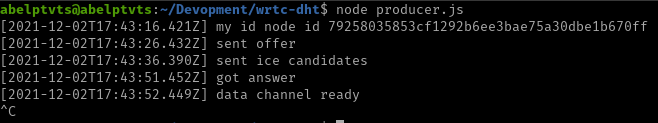
\includegraphics[width=120mm, keepaspectratio]{figures/producer}
    \caption{A termelő futás közben}
    \label{fig:prod}
\end{figure}

\begin{figure}[!ht]
    \centering
    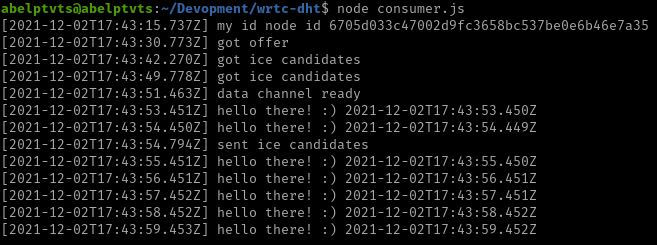
\includegraphics[width=120mm, keepaspectratio]{figures/consumer}
    \caption{A fogyasztó futás közben}
    \label{fig:cons}
\end{figure}


\section{Cache invalidáció}\label{sec:cache-invalidáció}
A DHT-be történő írás során a publikus tracker-ök meghatározatlan ideig tárolják az hozzájuk érkező adatokat.
Emiatt ha a proof-of-concept implementáció újraindul, a csatlakozás nem tud létrejönni, mivel a két fél a folyamatos
lekérdezés során elavult WebRTC offer-eket kap.
Az elvárt működéshez szükséges az, hogy a bucket-ek teljesen üresek legyenek.
Ezt a problémát oldja meg a Signalig osztály cacheBurst paramétere.
A cacheBurst paraméter egy szám, ami minden salt-ban szerepel, így garantálva, hogy az implementáció teljesen új bucket-eket
használ induláskor.
A proof-of-concept implementáció használata során a cacheBurst paramétert \emph{manuálisan} kell állítani.

%TODO possible improvements
    \chapter{Továbbfejlesztési lehetőségek}\label{ch:továbbfejlesztési-lehetőségek}

A jelenlegi algoritmus legszembetűnőbb hiánya az, hogy csupán két fél tud egymással kommunikálni.
Alapvetően ahhoz, hogy egy csomópont kommunikálni tudjon egy másikkal, az szükséges, hogy ismerjék egymás kulcspárának
publikus részét.
Ezt jelenleg kézzel kell konfigurálni.
A konfigurálandó kulcsok száma a választott hálózati topológiától függ.
Értelemszerűen ez a szám a \emph{full mesh} topológia esetében lesz a legnagyobb, és több ezer csomópont esetén nem fenntartható
az, hogy manuálisan legyen szükséges konfigurálni a kulcsokat minden csomóponton.
Célszerű lehet az algoritmus oly módon módosítani, hogy minimális konfigurációval létre lehessen hozni egy full mesh
hálózatot.

\begin{figure}[!ht]
    \centering
    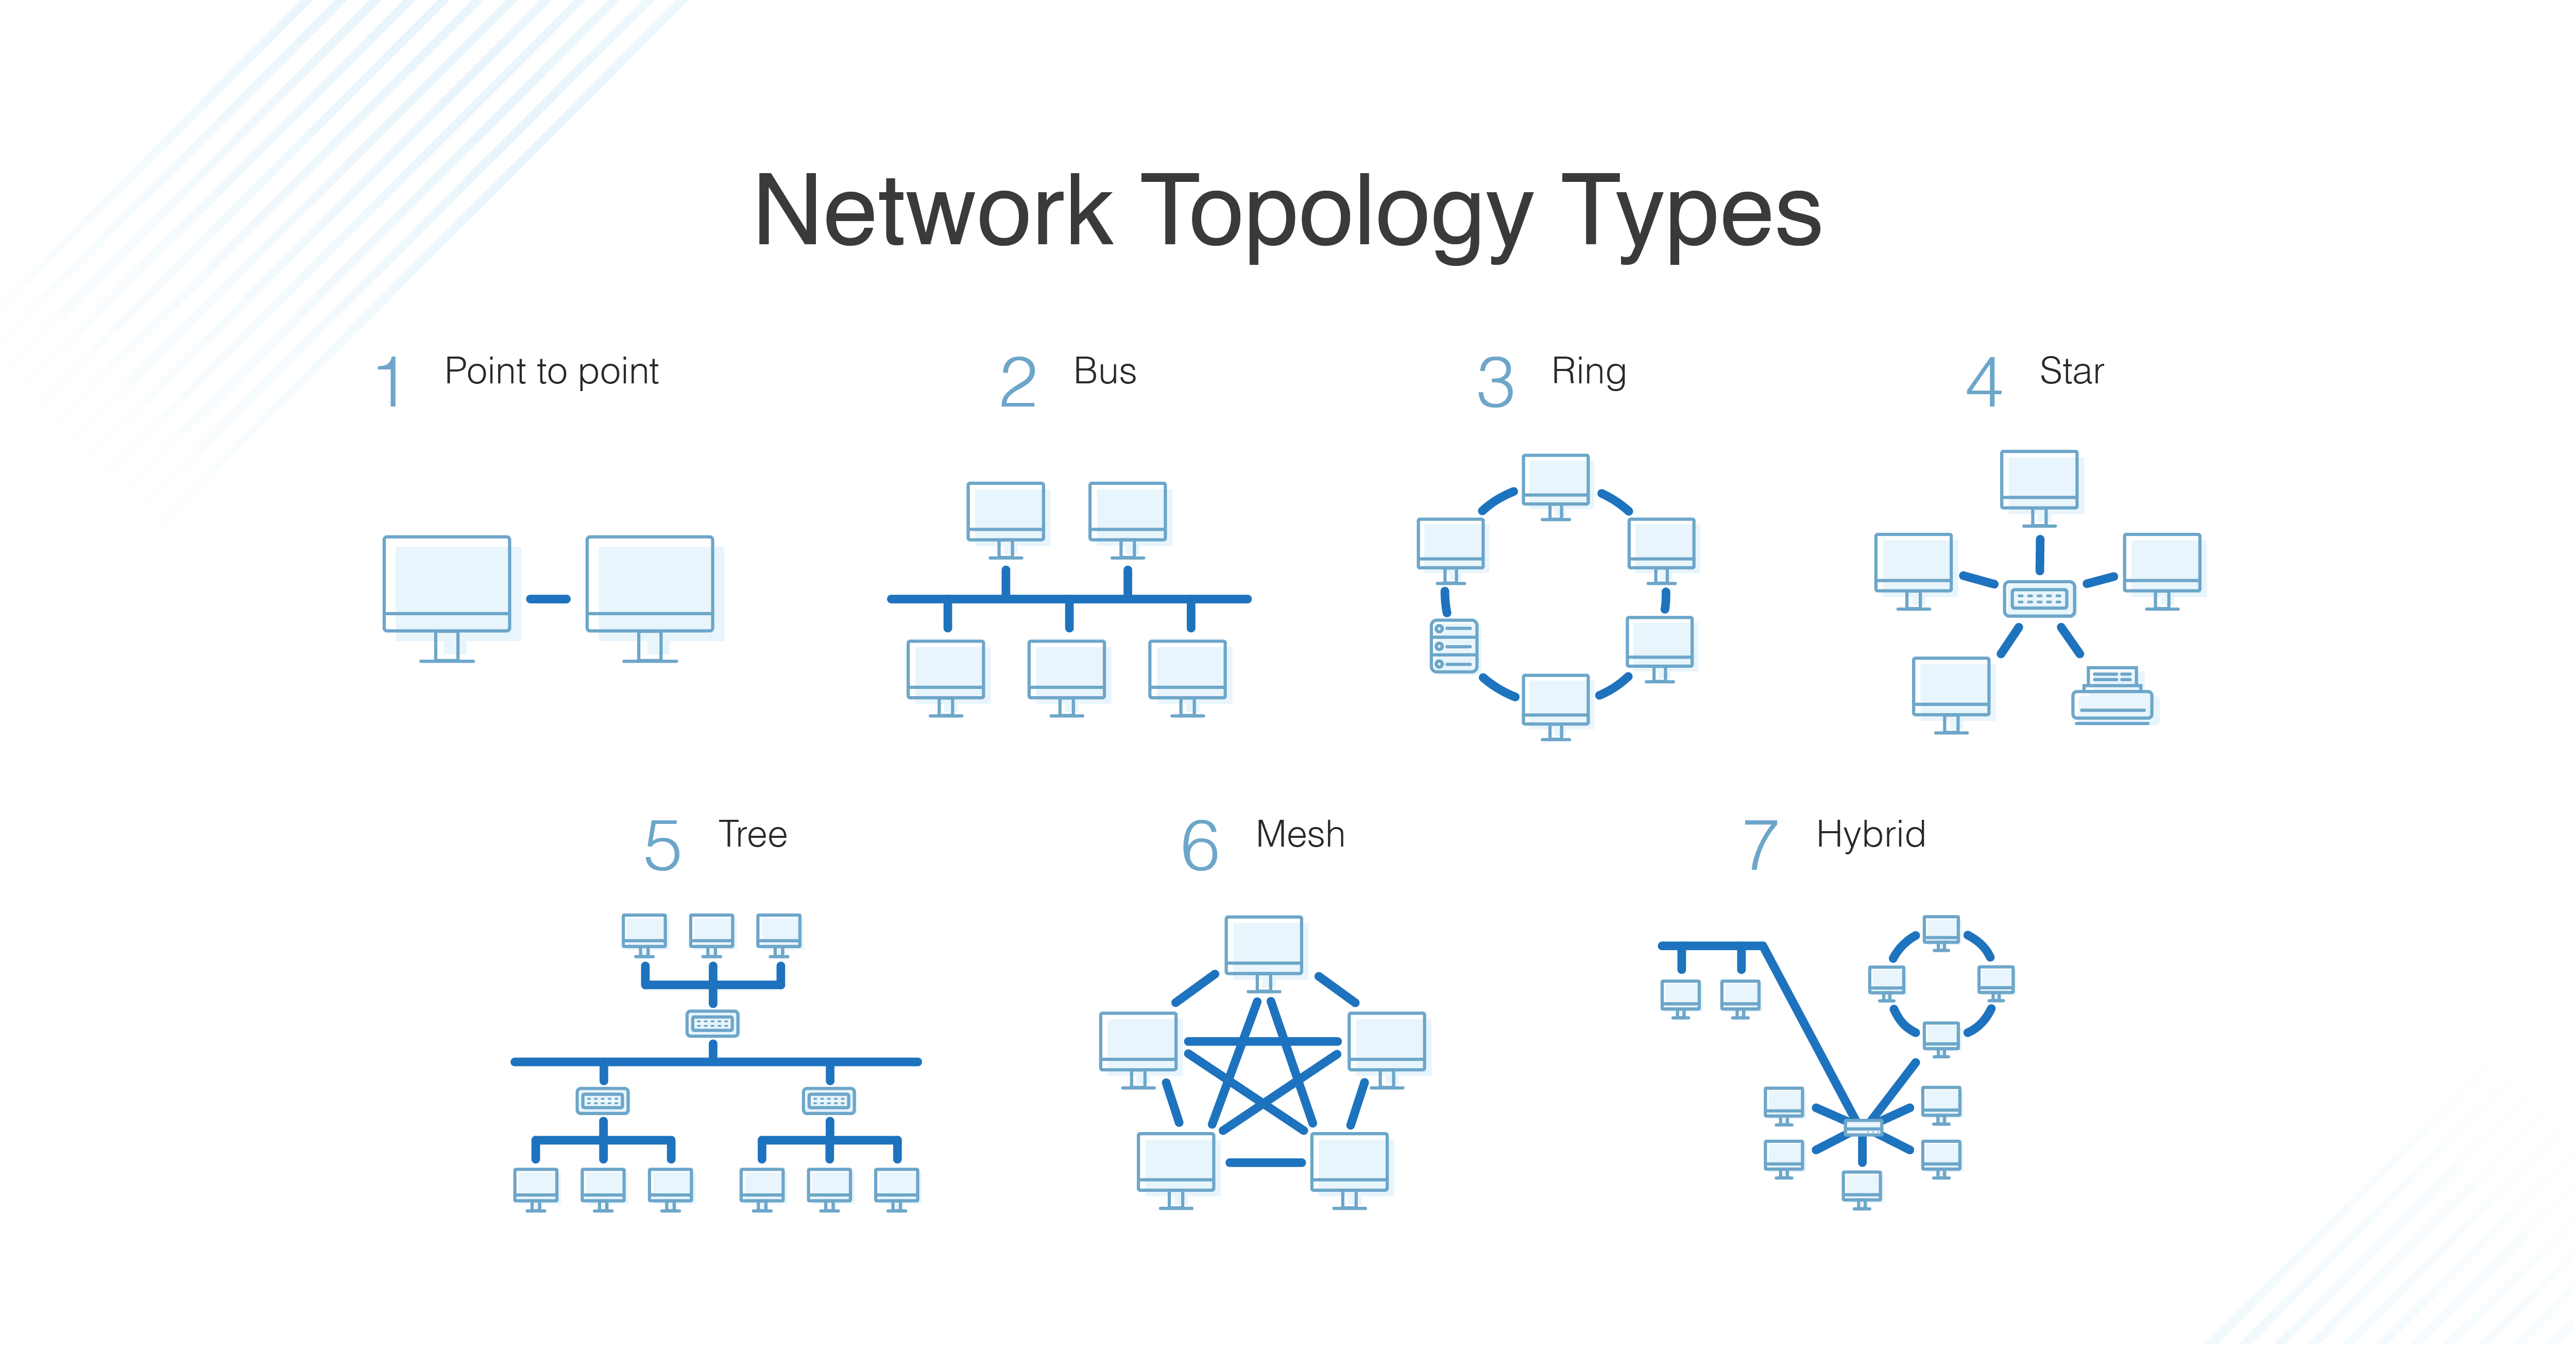
\includegraphics[width=140mm, keepaspectratio]{figures/topology}
    \caption{Különböző hálózati topológiák ábrázolva (forrás: https://www.dnsstuff.com/what-is-network-topology).}
    \label{fig:topo}
\end{figure}

Emellett ahhoz, egy csomópont több másikhoz tudjon csatlakozni, szükséges az, hogy minden általa a DHT-ba írt adat címzett
legyen.
Jelenleg ha több csomópont olvasná egy adott fél offers bucket-jét, akkor ezek nem tudnák eldönteni, hogy egy adott WebRTC
offer nekik, vagy épp egy másik csomópontnak lett szánva.
Ezen segíthet minden üzenet bővítése a célzott csomópont DHT-beli egyedi azonosítójával vagy publikus kulcsával.

Jelenleg a csomópontok által írt bucket-ek a publikus interneten vannak tárolva, és bár kellően nagy a publikus kulcsok
entrópiája ahhoz, hogy ne lehessen konfiguráció nélkül csatlakozni egy félhez, ez komoly biztonsági rést jelenthet.
Ahhoz, hogy ezt elkerüljük, célszerű lehet titkosítani a DHT bucket-ekbe írt adatokat.


% List of Figures, Tables
%~~~~~~~~~~~~~~~~~~~~~~~~~~~~~~~~~~~~~~~~~~~~~~~~~~~~~~~~~~~~~~~~~~~~~~~~~~~~~~~~~~~~~~
%\listoffigures\addcontentsline{toc}{chapter}{\listfigurename}
%\listoftables\addcontentsline{toc}{chapter}{\listtablename}


% Bibliography
%~~~~~~~~~~~~~~~~~~~~~~~~~~~~~~~~~~~~~~~~~~~~~~~~~~~~~~~~~~~~~~~~~~~~~~~~~~~~~~~~~~~~~~
    \addcontentsline{toc}{chapter}{\bibname}
    \bibliography{bib/mybib}
    \label{page:last}
\end{document}
